\documentclass[../review_3.tex]{subfiles}
\graphicspath{{\subfix{../img/}}}
\begin{document}

\chapter{Softwaremetriken und Statistiken}\thispagestyle{fancy}
Der Zweck von Softwaremetriken besteht in der ,,Definition von Software-Kenngrößen und Entwicklungsprozessen'' und der ,,Abschätzung des Prozess- und Kostenaufwands oder dem Qualitätsmanagement''\cite{swmetriken}.

Da das Reviewdokument noch vor Projektende fertiggestellt werden musste, sind die Daten, auf denen dieses Kapitel basiert, vom 10.07.2021.
\section{Benennungs- und Programmierkonventionen}
Während der Meetings wurde sich auf zahlreiche Konventionen geeinigt. Diese wurden dann wiederum sowohl in den einzelnen Meetingprotokollen als auch in einem eigenen Wikieintrag festgehalten.

Unter Programmierkonventionen werden ,,Vorgaben für Programmierer über die Gestaltung von Programmen''\cite{progkonv} verstanden. Sie zeigen auf, wie der Code sowohl formal als auch strukturell gestaltet sein soll. Diese Konventionen sollen zur Verbesserung der Softwarequalität führen, was sich unter anderem in der durch die Konventionen gesteigerten Verständlichkeit und Änderungsfreundlichkeit des Codes zeigt.

\subsection{C/C++ und UML}
Das System wird in der Programmiersprache C++ entwickelt. Um dieses System zu entwerfen, wurden verschiedene Modelle und Diagramme im Rahmen des Softwareprojektes erstellt (z.B. Klassendiagramme, Aktivitätsdiagramme, Sequenzdiagramme). Diese Diagramme wurden mithilfe der Unified Modeling Language (UML) entwickelt. Die UML gibt bereits einige Richtlinien vor, wie zum Beispiel die grafische Notation oder die Bezeichner für die bei einer Modellierung wichtiger Begriffe.

\subsubsection{Namenskonventionen}
Im Folgenden werden die Namenskonventionen im vorliegenden Softwareprojekt aufgezeigt und mit kurzen Beispielen unterlegt:

\textbf{Klassen}, \textbf{Enumerations} und \textbf{Pakete} werden entsprechend der UpperCamelCase-Schreibweise dargestellt. Allerdings muss darauf geachtet werden, dass z. B. bei Akronymen nicht mehrere Buchstaben hintereinander in Großbuchstaben geschrieben werden.
Dementsprechend entspricht der Name \texttt{ConfigurationManagement} den Konventionen. Allerdings ist \texttt{TCPTreatment} syntaktisch nicht korrekt, da es den Vorgaben nicht entspricht, der Begriff \texttt{TcpTreatment} hingegen wäre syntaktisch korrekt.

Für \textbf{Methoden} werden ausschließlich Kleinbuchstaben verwendet. Sollte sich der Methodenname aus mehreren Worten zusammensetzen, kann dies über einen Unterstrich erfolgen. Beispiele für richtig benannte Methoden sind demzufolge \texttt{send\_packets\_to\_port()} und \texttt{check\_syn\_cookie()}. Es bleibt anzumerken, dass statische Methoden durch ein \texttt{s\_} vor dem eigentlichen Namen gekennzeichnet werden, wie bei \texttt{s\_increment\_timestamp()}.

Für \textbf{Variablen} gelten die gleichen Konventionen wie für Methoden, sodass \texttt{packet\_inside} als Bespiel dienen kann. Zusätzlich soll ein Unterstrich vor dem Namen darauf hinweisen, dass es sich um eine Membervariable handelt, wie z. B. bei \texttt{\_cookie\_secret}. Statische Membervariablen beginnen somit mit \texttt{\_s\_}, wie bei \texttt{\_s\_timestamp}.

Auch bei \textbf{Objekten} gilt, dass nur Kleinbuchstaben verwendet werden sollen und mehrere Worte durch einem Unterstrich verbunden werden, wie in \texttt{nic\_man}.

\subsubsection{Formatierungs-Richtlinien}
Die Formatierungsrichtlinien legen unter anderem fest, dass nur ASCII-Zeichen, also zum Beispiel keine Umlaute oder  ß, verwendet werden dürfen. Die Einrückung im Code beträgt vier Leerzeichen. Zudem sollen ,,dauerhaft'' geschweifte Klammern verwendet werden. Das heißt zum Beispiel, dass auch geschweifte Klammern einzeiliger if-Blöcken verwendet werden. Nach Methoden- und Klassennamen (oder Ähnlichem) stehen öffnende geschweifte Klammer. Hier soll kein Zeilenumbruch entstehen. Dies zeigt der Codeausschnitt \ref{klammern} beispielhaft.
\begin{lstlisting} [caption= {Formatierungsrichtlinie: Setzen von Klammern}, label = {klammern}]
int i = rand();
         
// It should be like this:
if(i%2 == 0){
    ...
}
         
//It should be not like this:
if(i%2 != 0)
{
    ...
}

//And not like this:
if(i>100)
    ...\end{lstlisting}

\subsubsection{Kommentare}
Während in den Kommentaren das Festschreiben von ToDo's erlaubt ist, dürfen hier keine Fragen gestellt werden. In den Headerdateien soll die Doxygen-Syntax für Kommentare verwendet werden, um hiermit unter anderem die Entwicklerdokumentation zu generieren. Vor einem Block können mehrzeilige Kommentare verwendet werden. Derjenige Teil, der mit \texttt{*} beginnt, muss jeweils nochmals mit einem Leerzeichen eingerückt werden.
\begin{lstlisting} [caption= {Beispiel für einen mehrzeiligen Doxygen-Kommentar}]
 /**
* Full description
*
* @brief short description
* @param msg message that is printed to the console
*/
void log(const string* msg){
    std::cout << msg << std::endl;
} \end{lstlisting}
Einzeilige Kommentare werden dadurch erzeugt, indem hinter einer Codezeile \texttt{///<} eingegeben wird. Diese Art von Kommentaren wird von Doxygen als Kurzbeschreibung verwendet.
\begin{lstlisting} [caption= {Beispiel für einen einzeiligen Doxygen-Kommentar}]
string firstname;  //< first name of person
string lastname;   //< last name of person
\end{lstlisting}

Es wurde sich auf die Verwendung folgender \textbf{Commands} geeinigt:

Bei \texttt{@brief} lässt sich sofort erkennen, dass es sich um eine \textbf{Kurzbeschreibung} handelt.

\texttt{@param} leitet hingegen die Beschreibung eines \textbf{Parameters}, der in eine Methode ein- oder von einer Methode ausgegeben wird, ein. \texttt{@param[in]} steht vor der Beschreibung eines \textbf{Eingabeparameters} und \texttt{@param[out]} vor einem \textbf{Ausgabeparameter}. Bei diesem handelt es sich um einen Parameter, der im C-Style einer Funktion mit Call-by-reference übergeben wird, damit er mit Werten gefüllt wird. Zur Beschreibung von Parametern, die sowohl ein- als auch ausgegeben werden, kann \texttt{@param[in, out]} verwendet werden.

Der Command \texttt{@return} hilft bei der Beschreibung eines \textbf{Rückgabewertes} und \texttt{@file} zur Erklärung des \textbf{Zwecks} einer Datei, also z. B. einer Klasse oder eines structs.

\subsubsection{Source-Dateien}
Pro Paket (vgl. Abb. \ref{fig:dospaketdiagramm}) wird ein Ordner in \texttt{source/} angelegt, der den gleichen Namen wie das Paket erhält. Alle zu diesem Paket zugehörigen Klassen befinden sich dann wiederum in diesem Ordner. Pro cpp-Klasse soll es eine eigene .cpp-Datei geben. Die dazugehörige Header-Datei  wird mit \texttt{\#include <header-file>} inkludiert. Im ganzen Projekt gibt es eine \texttt{main.cpp}-Datei in \texttt{source/} mit der main-Routine.

\subsubsection{Header-Dateien}
Pro Source-Datei existiert eine Header-Datei. Jede dieser Header-Dateien wird mit \texttt{.hpp} benannt. Am Anfang der Datei wird \texttt{\#pragma once} verwendet. Externe Dateien werden mit \texttt{\#include <file>} inkludiert.

\subsection{Gitlab}
Im Softwareprojekt wird die GitLab zur Versionsverwaltung genutzt. Diese Webanwendung basiert auf Git.

\subsubsection{Git}
Außer in Präsentationen und Review-Dokumenten werden in Git nur ASCII-Zeichen verwendet. Die \textbf{Sprache} ist auch hier grundsätzlich Englisch, wobei diese Festlegung auch bei den Präsentationen und Review-Dokumenten abweicht.

Die \textbf{Branchnamen} sind klein geschrieben. Die Worte in diesem werden mit Unterstrich (,,\_'') verbunden. Dieselbe Regelungen gelten bei \textbf{Ordner- und Dateinamen}.

\subsubsection{Issue}
Grundsätzlich werden die Issues in Englisch benannt. Lediglich deutsche ,,Eigennamen'' werden auf Deutsch geschrieben (Beispiel: Pflichtenheft).
Die Issues werden klein und im Imperativ geschrieben. Leerzeichen sind erlaubt.

Wenn Issues nicht nur einer sondern mehreren Personen zugeordnet werden sollen, wird dem eigentlichen Issue-Namen mit ,,@'' die Namen der zuständigen Teammitgliedern angehängt. Das heißt, der Issue-Name weist folgende Struktur auf: \texttt{<issue name> <space> @ <first name>}).

Mit \texttt{@all} ist das Issue für alle Teammitglieder für die Bearbeitung offen. Derjenige, der mit der Bearbeitung dieser Aufgabe beginnt, löscht ,,@all'' trägt seinen eigenen Vornamen mit ,,@'' in den Issue-Namen ein.

\subsubsection{Label}
In diesem Projekt werden die Labels grundsätzlich für zwei verschiedene Kategorien von Aufgaben verwendet verwendet: Zum einen für Status-Issues und zum anderen für Super-Issues (bzw. Tasks). Bei diesen Super-Issues handelt es sich um große Aufgaben, denen wiederum verschiedene Issues als Teilaufgaben zugeordnet werden.

Die Benennung sieht Folgendes vor:

\begin{figure} [h]
    \centering
    
\includegraphics[width = 0.2\linewidth]{img/status.png}
    \caption{Beispiel: Label für Status-Issus}
    \label{status}
\end{figure}
Label für \texttt{Status-Issues} werden folgendermaßen benannt: \texttt{STATUS: <label name>}. Diese werden zur Darstellung auf dem Issue-Board verwendet. \texttt{STATUS: in process} (siehe Abb. \ref{status}) und \texttt{STATUS: to be tested or presented} sind Beispiele für diese Status-Issues.

\begin{figure} [h]
    \centering
    
\includegraphics[width = 0.26\linewidth]{img/task.png}
    \caption{Beispiel: Label für Super-Issus/ Tasks}
    \label{task}
\end{figure}
Label für \texttt{Super-Issues bzw. Tasks} werden folgendermaßen benannt: \texttt{TASK <label name>}. Jedes Issue soll genau einem Ticket zugeordnet werden, um zu erkennen, welcher großen Aufgabe das Issue zugehört. Ein Beispiel für ein solches Label findet sich in Abbildung \ref{task}.

\begin{figure} [h]
    \centering
    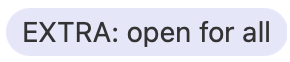
\includegraphics[width = 0.23\linewidth]{img/extra.png}
    \caption{Beispiel: Label für außerordentliche Kategorien}
    \label{extra}
\end{figure}
Label, die keiner dieser beiden Kategorien zugeordnet werden könne, werden folgendermaßen benannt: \texttt{EXTRA: <label name>}. Als Beispiel hierfür kann das Label \texttt{EXTRA: open for all} genannt werden, welches es den Teammitgliedern verinfachen soll, noch nciht zugeteilte Aufgaben zu finden.

\subsection{Latex}
Zum Erstellen der Reviewdokumente und der Präsentationen wird Latex verwendet. Hierbei wurde sich darauf geeinigt, unter anderem um Merge-Konflikte zu verhindern, dass ein Tab vier Leerzeichen entspricht. Außerdem sollen neue Kapitel mit einem Kommentarblock eingeleitet werden, um sich besser in den Dokumenten zurechtzufinden.


\section{Umfang der Software}

Unter \textbf{Lines of Code} (Loc) wird die Anzahl der Zeilen inklusive Leerzeilen und Kommentare verstanden. Dagegen enthalten die \textbf{Source Lines of Code} (SLOC) nur Codezeilen ohne Leerzeilen und Kommentare. Die \textbf{Comment Lines of Code} (CLOC) geben die Anzahl der Kommentarzeilen an. Dabei werden in diesem Dokument in diese Zeilenanzahl keine Zeilen miteinbezogen, welche zugleich Code und Kommentaren beinhalten.

Die Lines of Codes von allen Header-Dateien betragen ungefähr 2000. Das davon über die Hälfte Kommentarzeilen sind, überrascht nicht. Denn die gesamte Codedokumentation bzw. Entwicklerdokumentation erfolgte in diesem Projekt mittels Doxygen, was die automatische Generierung von Dokumentation auf Basis spezieller Kommentare. Diese Dokumentation mittels Kommentarzeilen fand in den Header-Dateien statt.
\begin{longtable}[H]{p{10cm}rrr}
    \toprule
    \textbf{Header-Datei}   & \textbf{LOC} & \textbf{CLOC} & \textbf{SLOC} \\ \midrule \endhead
    AttackThread.h          & 91           & 25            & 44            \\
    Cli.h                   & 32           & 2             & 24            \\
    Configurator.h          & 114          & 58            & 45            \\
    DebugHelper.h           & 10           & 0             & 7             \\
    DefenseThread.h         & 36           & 17            & 13            \\
    Definitions.h           & 24           & 7             & 9             \\
    ForwardingThread.h      & 30           & 14            & 11            \\
    Initializer.h           & 52           & 27            & 18            \\ %eigner Branch?
    Inspection.h            & 149          & 107           & 33            \\
    NetworkPacketHandler.h  & 62           & 44            & 13            \\
    PacketContainer.h       & 320          & 235           & 55            \\
    PacketInfo.h            & 82           & 38            & 26            \\
    PacketInfoCreator.h     & 43           & 18            & 18            \\
    PacketInfoIpv4.h        & 79           & 39            & 25            \\
    PacketInfoIpv4Icmp.h    & 39           & 17            & 14            \\
    PacketInfoIpv4Tcp.h     & 156          & 99            & 35            \\
    PacketInfoIpv4Udp.h     & 56           & 27            & 18            \\
    PacketInfoIpv6Icmp.h    & 36           & 7             & 22            \\
    PacketInfoIpv6Tcp.h     & 71           & 21            & 41            \\
    PacketInfoIpv6Udp.h     & 39           & 7             & 26            \\
    PacketProtTcp.h         & 138          & 89            & 31            \\
    PacketProtUdp.h         & 31           & 16            & 11            \\
    rand.h                  & 42           & 19            & 16            \\
    RandomNumberGenerator.h & 56           & 33            & 16            \\
    StatisticsThread.h      & 43           & 0             & 34            \\ %hier könnten noch Änderungen in anderem Branch sein
    Thread.h                & 20           & 6             & 10            \\
    Treatment.h             & 215          & 129           & 54            \\ \midrule
    $\sum$                  & 2066         & 1101          & 669           \\ \bottomrule
\end{longtable}

Von den insgesamt über 2500 LoC in den Source-Dateien sind ca. 13,25\% Kommentarzeilen und ca. 67,41\% Codezeilen ohne Kommentare und Leerzeilen.
\begin{longtable}[H]{p{10cm}rrr} \toprule
    \textbf{Source-Datei}    & \textbf{LoC} & \textbf{CLOC} & \textbf{SLOC} \\ \midrule \endhead
    Attacker/main.cpp        & 103          & 10            & 67            \\
    AttackThread.cpp         & 206          & 13            & 150           \\
    Cli.cpp                  & 102          & 18            & 57            \\%toDo
    Configurator.cpp         & 95           & 12            & 69            \\
    DebugHelper.cpp          & 64           & 9             & 43            \\
    DefenseThread.cpp        & 68           & 17            & 31            \\
    ForwardingThread.cpp     & 6            & 0             & 5             \\
    Initializer.cpp          & 249          & 29            & 181           \\
    Inspection.cpp           & 145          & 22            & 109           \\
    main.cpp                 & 106          & 10            & 69            \\
    NetworkPacketHandler.cpp & 41           & 1             & 32            \\
    PacketContainer.cpp      & 230          & 5             & 168           \\
    PacketInfo.cpp           & 73           & 18            & 38            \\
    PacketInfoCreator.cpp    & 149          & 9             & 116           \\
    PacketInfoIpv4.cpp       & 57           & 0             & 44            \\
    PacketInfoIpv4Icmp.cpp   & 18           & 0             & 14            \\
    PacketInfoIpv4Tcp.cpp    & 110          & 3             & 77            \\
    PacketInfoIpv4Udp.cpp    & 30           & 0             & 23            \\
    PacketInfoIpv6Icmp.cpp   & 36           & 11            & 18            \\
    PacketInfoIpv6Tcp.cpp    & 60           & 11            & 34            \\
    PacketInfoIpv6Udp.cpp    & 50           & 11            & 30            \\
    PacketProtTcp.cpp        & 88           & 1             & 71            \\
    PacketProtUdp.cpp        & 10           & 0             & 7             \\
    StatisticsThread.cpp     & 55           & 10            & 34            \\ %nochmal in den Branch schauen
    Thread.cpp               & 5            & 0             & 3             \\
    Treatment.cpp            & 394          & 118           & 229           \\ \midrule
    $\sum$                   & 2550         & 338           & 1719          \\ \bottomrule
\end{longtable}

Die Test-Dateien beinhalten den Code der Unit-Tests. Über die Hälfte der LOC aller Test-Dateien kommen aus der Datei \texttt{Treatment\_test.cpp}.
In den Test-Dateien wurdemusste vergleichsweise wenig kommentiert werden, wenn die Namen der Testcases und der Sections aussagekräftig gewählt wurden und diese Aussagekraft durch die Strukturierung der Tests unterstützt wurde.
\begin{longtable}[H]{p{10cm}rrr} \toprule
    \textbf{Test-Datei}             & \textbf{LoC} & \textbf{CLOC} & \textbf{SLOC} \\ \midrule \endhead
    Attacker\_test.cpp              & 37           & 7             & 24            \\
    Configurator\_test.cpp          & 52           & 0             & 43            \\
    Inspection\_test.cpp            & 15           & 0             & 23            \\
    libdpdk\_dummy\_test.cpp        & 14           & 0             & 11            \\
    PacketContainer\_test.cpp       & 299          & 4             & 237           \\
    PacketInfo\_test.cpp            & 131          & 57            & 62            \\ %noch vieles auskommentiert
    RandomNumberGenerator\_test.cpp & 456          & 106           & 315           \\
    Treatment\_test.cpp             & 1170         & 95            & 846           \\  \midrule
    $\sum$                          & 2174         & 268           & 1561          \\ \bottomrule
\end{longtable}

Die lipdpdk-Header-Dateien wurden hier extra aufgeführt, da sie nicht komplett selbst geschrieben wurden, sondern vor allem durch Kopieren und Anpassung entstanden sind.
\begin{longtable}[H]{p{10cm}rrr} \toprule
    \textbf{lipdpdk\_dummy-Header-Datei} & \textbf{LoC} & \textbf{CLOC} & \textbf{SLOC} \\ \midrule \endhead
    rte\_branch\_prediction.h            & 33           & 20            & 9             \\
    rte\_byteorder.h                     & 62           & 20            & 31            \\
    rte\_common.h                        & 14           & 0             & 12            \\
    rte\_config.h                        & 3            & 0             & 2             \\
    rte\_cycles.h                        & 14           & 1             & 10            \\
    rte\_eal.h                           & 1            & 0             & 1             \\
    rte\_ethdev.h                        & 44           & 20            & 20            \\
    rte\_ether.h                         & 23           & 0             & 18            \\
    rte\_icmp.h                          & 12           & 0             & 10            \\
    rte\_ip.h                            & 139          & 7             & 109           \\
    rte\_lcore.h                         & 3            & 0             & 2             \\
    rte\_mbuf.h                          & 136          & 4             & 104           \\
    rte\_mbuf\_core.h                    & 8            & 0             & 5             \\
    rte\_mempool.h                       & 3            & 0             & 2             \\
    rte\_tcp.h                           & 16           & 0             & 14            \\
    rte\_udp.h                           & 10           & 0             & 8             \\ \midrule
    $\sum$                               & 527          & 72            & 357           \\ \bottomrule
\end{longtable}
Um das Testbed effizient nutzen zu können, wurden kurze Skripte zur Initialisierung der Hardware geschrieben. Insgesamt entstanden hierbei 26 LoC.
\begin{longtable}[H]{p{10cm}rrr} \toprule
    \textbf{Skripte zur Intialisierung der Hardware} & \textbf{LoC} & \textbf{CLOC} & \textbf{SLOC} \\ \midrule \endhead
    namespace\_bob.sh                                & 13           & 6             & 7             \\
    namespace\_alice.sh                              & 13           & 6             & 7             \\
    \midrule
    $\sum$                                           & 26           & 12            & 14            \\ \bottomrule
\end{longtable}
Insgesamt entstanden im vorliegenden Projekt ca. 7300 LOC, fast 1800 CLOC und ca. 4300 SLOC.
\begin{longtable} [H]{p{10cm}rrr}
    \toprule
    \textbf{Datei-Art}                       & \textbf{LoC} & \textbf{CLOC} & \textbf{SLOC} \\ \midrule \endhead
    Header-Dateien                           & 2066         & 1101          & 669           \\
    Source-Dateien                           & 2550         & 338           & 1719          \\
    Test- Dateien                            & 2174         & 268           & 1561          \\
    lipdpdk\_dummy-Header-Dateien            & 527          & 72            & 357           \\
    Skripte zur Initialisierung der Hardware & 26           & 12            & 14            \\\midrule
    $\sum$                                   & 7343         & 1791          & 4320          \\ \bottomrule
\end{longtable}

\section{Repository-Analyse in Gitlab}
Ein Teil der Funktionalität von Gitlab bilden die Repository-Analysen. Diese werden verwendet, um sich  einen stark abstrahierten Überblick über das Git-Repository eines Projektes zu verschaffen. Die dort zur Verfügung gestellten Diagramme werden nach jedem Commit aktualisiert.
\subsection{Verwendete Programmiersprachen}
\begin{figure} [h]
    \centering
    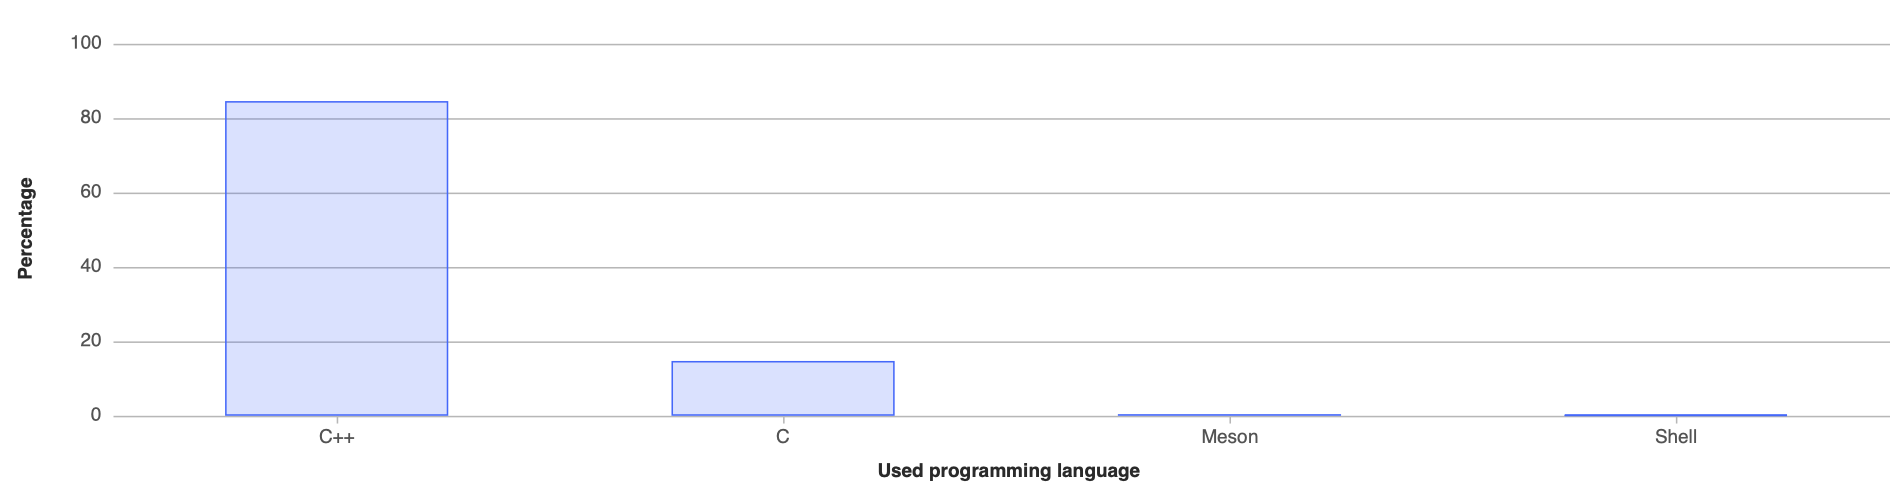
\includegraphics[width =0.95\linewidth]{img/gitlab1.png}
    \caption{Verwendete Programmiersprachen in Prozent, gemessen an den Bytes of Code}
    \label{gitlab1}
\end{figure}
Abbildung \ref{gitlab1} zeigt, dass im Repository des vorliegenden Softwareprojektes  vorwiegend mit 84,6\% die Programmiersprache C++ verwendet wurde. Mit großen Abstand folgt C mit 14,74\%. Der C-Code resultiert aus die Beispielprogramme von DPDK, die verwendet werden, um die Funktionalität von DPDK zu testen. Diese Beispielprogramme werden in dem Repoisitory, das später auf Github veröffentlicht wird, nicht mehr vorhanden sein. Meson (0,44\%) und Shell (0,23\%) stellen keinen wesentlichen Anteil dar.
\subsection{Commit-Statistik}
Insgesamt gab es vom 03.05.2021 bis zum 08.07.2021 im Master-Branch 1183 Commits. Merge-Commits sind hierbei ausgeschlossen. Aus diesen Zahlen lässt sich folgern, dass es durchschnittlich 17,7 Commits pro Tag gab.
\begin{figure} [h]
    \centering
    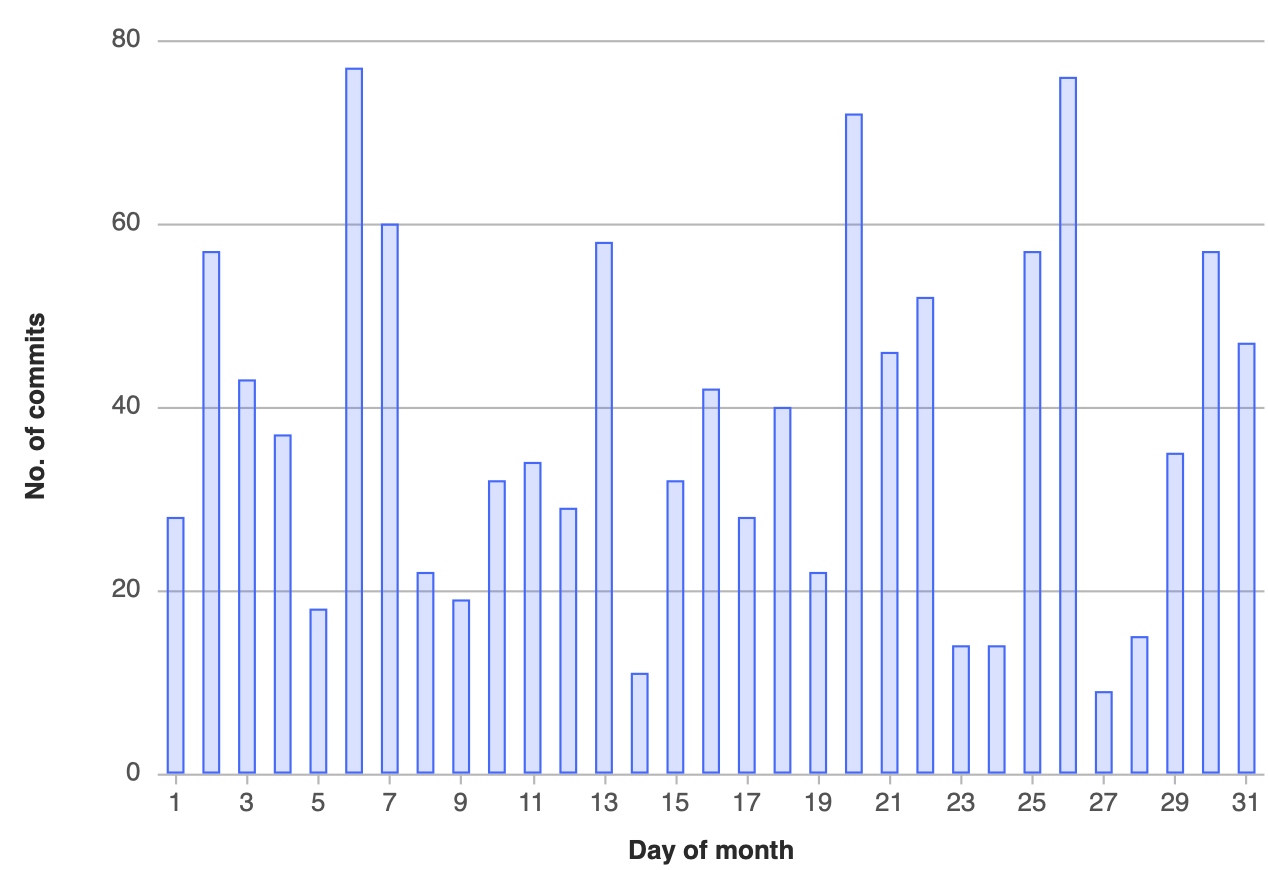
\includegraphics[width =0.65\linewidth]{img/gitlab2.png}
    \caption{Commits pro Tag des Monats, Zeitraum: 03.05.2021 bis 08.07.2021}
    \label{gitlab2}
\end{figure}
Abbildung \ref{gitlab2} macht deutlich, das die Anzahl der Commits pro Tag des Monats stark schwankte. An manchen Tagen gab es weniger als 10 Commits (z.B. Tag 27), an anderen beinahe 80 (z.B. Tag 7, Tag 26).
\begin{figure} [h]
    \centering
    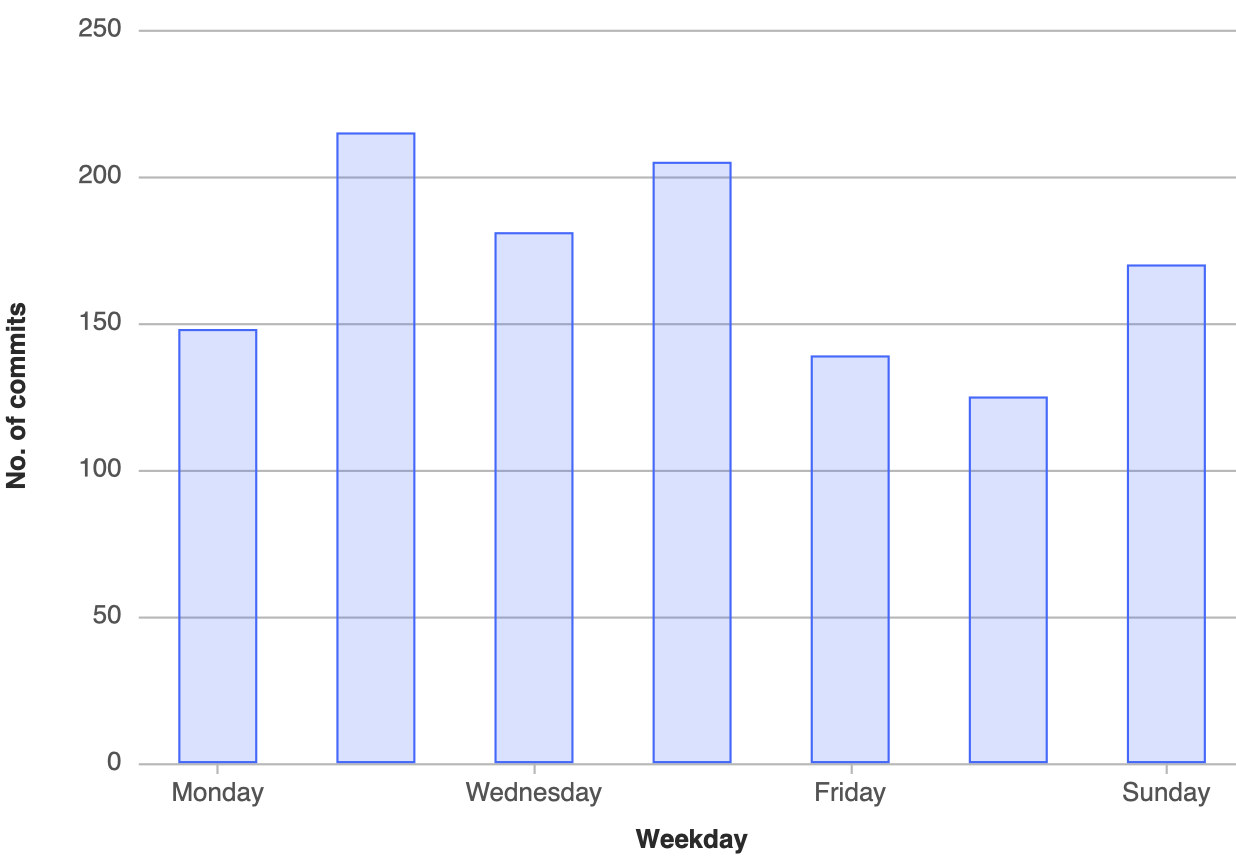
\includegraphics[width =0.55\linewidth]{img/gitlab3.png}
    \caption{Commits pro Wochentag (UTC), Zeitraum: 03.05.2021 bis 08.07.2021}
    \label{gitlab3}
\end{figure}
Abbildung \ref{gitlab3} zeigt, dass es dienstags die meisten Commits pro Wochentag gab (215 Commits pro Tag). Die Wochentage Donnerstag (205 Commits pro Tag), Mittwoch (181 Commits pro Tag), Sonntag (170 Commits pro Tag), Montag (148 Commits pro Tag) und Freitag (139 Commits pro Tag) folgen. Mit 125 Commits pro Tag gab es die wenigsten Commits samstags.
\begin{figure} [h]
    \centering
    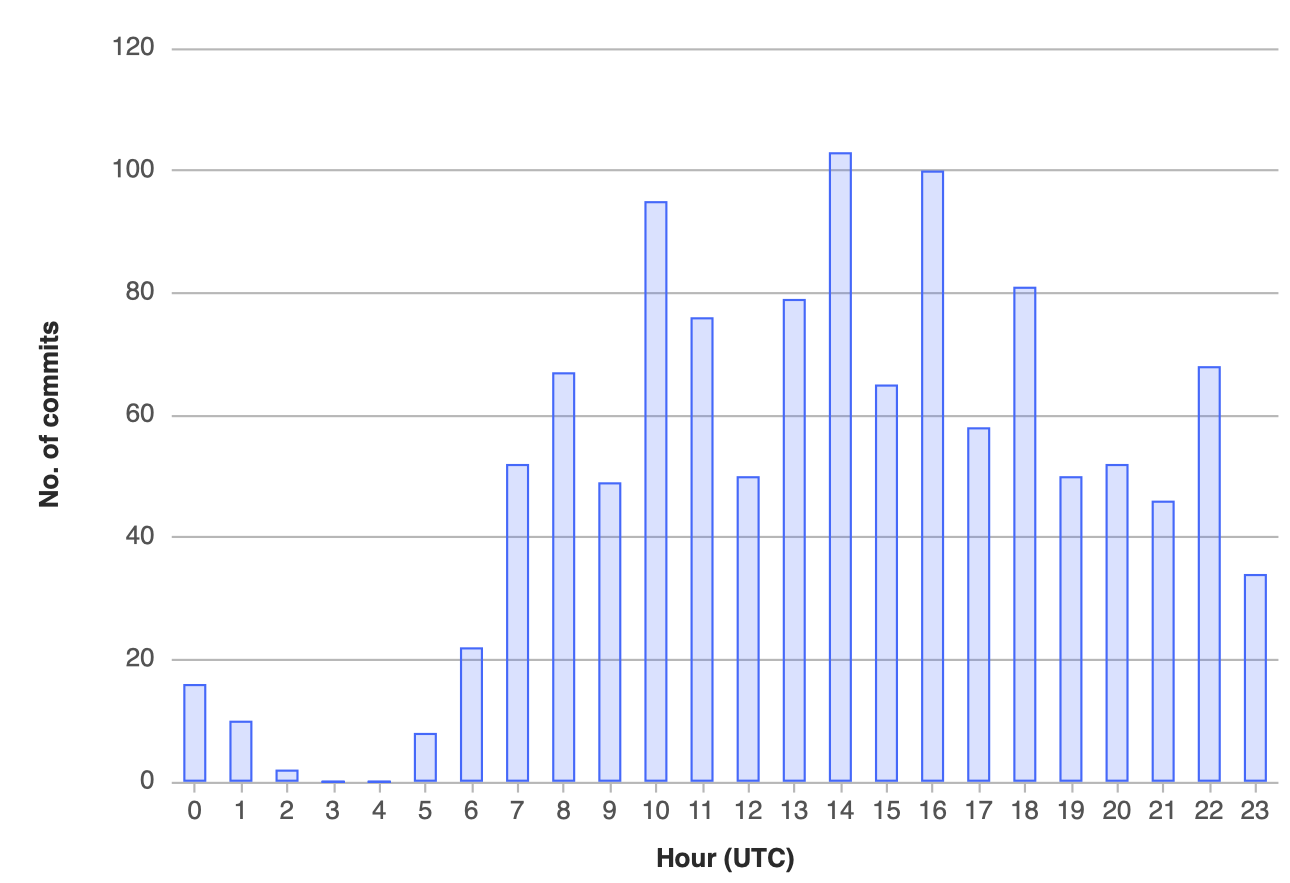
\includegraphics[width =0.65\linewidth]{img/gitlab4.png}
    \caption{Commits pro Stunde des Tages (UTC), Zeitraum: 03.05.2021 bis 08.07.2021}
    \label{gitlab4}
\end{figure}
In Abbildung \ref{gitlab4} sind die Commits pro Stunde des Tages dargestellt. Die Abbildung macht deutlich, dass kaum nachts gearbeitet wurde, insbesondere kaum zwischen 2 und 5 Uhr. Dagegen gab es vor allem am späten Vormittag bis späten Nachmittag viele Commits.

\end{document}
